% !TeX spellcheck = en_US
\documentclass[12pt]{article}
\usepackage[utf8]{inputenc}
\usepackage[spanish]{babel}
\usepackage{graphicx}
\usepackage[margin=2.5cm]{geometry}
\usepackage{float}



\usepackage[utf8]{inputenc}
\usepackage{amsmath}
\usepackage{amsfonts}
\usepackage{geometry}
\newcommand{\hrules}{\rule{\linewidth}{0.5mm}}

\begin{document}
	
	\begin{titlepage}
		\centering
		
		\begin{minipage}{0.2\textwidth}
			\begin{flushleft}
				
\includegraphics[width=\textwidth]{logo_ipn.png}
			\end{flushleft}
		\end{minipage}
		\hfill
		\begin{minipage}{0.5\textwidth}
			\centering
			{\scshape\Large Instituto Politécnico Nacional} \\[0.3cm]
			{\scshape\large Escuela Superior de Cómputo}
		\end{minipage}
		\hfill
		\begin{minipage}{0.2\textwidth}
			\begin{flushright}
				
\includegraphics[width=\textwidth]{logo_escom.png}
			\end{flushright}
		\end{minipage}
		
		\vspace{1.5cm}
		
		{\large\textbf{Ingeniería en Inteligencia Artificial}} \\[1.5cm]
		
		{\Large\textbf{Reconocimiento de voz}} \\[2cm]
		
		\hrules
		\vspace{0.4cm}
		{\huge\bfseries Actividad 1: Introducción
		} \\[0.4cm]
		\hrules
		\vspace{2.5cm}
		
		% --- INFORMACIÓN PERSONAL ---
		\begin{minipage}{0.8\textwidth}
			\begin{flushleft} \large
				\textbf{Profesor:} \\
				Enrique Alfonso Carmona García\\[1cm]
				
				\textbf{Alumno:} \\
				Velázquez Arrieta Eduardo Uriel
			\end{flushleft}
		\end{minipage}
		
		\vfill
		
		{\large Fecha de entrega: 2 de Septiembre 2026}
		
	\end{titlepage}
	
	
	\newpage
	\tableofcontents % Índice de contenido
	\vspace{1cm}
	\listoffigures    % Índice de imágenes
	\newpage
	
	
	\section{Desarrollo}
	\subsection{Preguntas de reflexión y análisis}
	
	\begin{itemize}
		\item ¿Cuál es la diferencia entre procesamiento de habla y procesamiento digital de señales en general?
		
		El reconocimiento de voz es una rama de la IA que se apoya en el PDS para poder procesar la onda de audio física. Mientras que el PDS se enfoca en la manipulación y transformación matemática de cualquier tipo de señal (filtrado, compresión, etc.), el procesamiento de habla busca extraer características específicas de la voz para que la computadora logre entender nuestras palabras y darles significado.
		
		\item Menciona al menos tres aplicaciones cotidianas del reconocimiento de voz.
		
		\begin{itemize}
			\item Resumen de reuniones en plataformas como Zoom o Teams.
			\item Uso de asistentes virtuales como Alexa, Cortana, Siri o Google Assistant.
			\item Dictado de texto en dispositivos móviles y traductores en tiempo real.
		\end{itemize}
		
		\item ¿Qué representa la probabilidad $P(W | O)$ en el contexto de un sistema de reconocimiento de voz?
		
		Representa la probabilidad a posteriori de que el locutor haya pronunciado la secuencia de palabras $W$ dado que el sistema observó la secuencia de características acústicas $O$ (el audio capturado). Es la probabilidad que el decodificador intenta maximizar para encontrar la transcripción correcta.
		
		\item Explica cómo el teorema de Bayes se aplica en el reconocimiento automático de voz. 
		
		Dado que calcular $P(W | O)$ directamente es complejo, el teorema de Bayes permite reescribir el problema como $P(W | O) = \frac{P(O | W) P(W)}{P(O)}$. Como $P(O)$ es igual para todas las secuencias candidatas, el sistema solo necesita maximizar el producto de $P(O | W)$ (proporcionado por el modelo acústico) y $P(W)$ (proporcionado por el modelo de lenguaje).
		
		\item ¿Qué función cumple el modelo acústico en un sistema de reconocimiento de voz?
		
		Se encarga de modelar la relación estadística entre los segmentos de audio (las observaciones $O$) y los fonemas o unidades fonéticas del idioma. En términos probabilísticos, estima $P(O | W)$, evaluando qué tan probable es que se genere una señal de audio específica si el usuario intentaba decir la palabra $W$.
		
		\item ¿Cuál es el papel del modelo de lenguaje en el reconocimiento de voz?
		
		Su función es estimar la probabilidad a priori $P(W)$ de que una secuencia de palabras ocurra en un idioma determinado. Proporciona el contexto sintáctico y semántico, ayudando al sistema a predecir qué palabras tienen sentido juntas y a desambiguar términos que suenan igual pero se escriben distinto (homófonos).
		
		\item Explica la importancia de la parte frontal acústica en la arquitectura de un sistema de reconocimiento de voz.
		
		La parte frontal acústica (o \textit{Front-End}) es crucial porque se encarga del preprocesamiento y la extracción de características. Captura la señal de audio cruda, elimina ruido y extrae vectores de características relevantes (como los coeficientes MFCC) que representan la información fonética de manera compacta, descartando información redundante para facilitar el trabajo del modelo acústico.
		
		\item ¿Qué diferencia hay entre un modelo paramétrico y un modelo no paramétrico?
		
		Un modelo paramétrico asume que los datos provienen de una distribución de probabilidad conocida (como una Gaussiana) y resume toda la información mediante un número fijo de parámetros (como la media y la varianza). Por el contrario, un modelo no paramétrico no asume una forma funcional predefinida y su complejidad o número de parámetros puede crecer en función de la cantidad de datos de entrenamiento.
		
		\item ¿En qué consiste la técnica de estimación de núcleo de Parzen dentro del modelado no paramétrico?
		
		Es un método para estimar la función de densidad de probabilidad de una variable aleatoria sin asumir una distribución paramétrica previa. Consiste en colocar una función de núcleo (kernel), como una campana de Gauss, centrada en cada punto de los datos de muestra. La densidad global se calcula sumando y promediando todas estas contribuciones individuales, creando una curva suave que se adapta a la forma real de los datos.
	\end{itemize}
	
	\subsection{Preguntas prácticas y de aplicación (ejercicios)}
	
	
	\begin{itemize}
		\item {Dibuja un esquema con los componentes principales de un sistema de reconocimiento de voz e indica su función.}
		
		\begin{itemize}
			\item{Entrada de audio:} 
			\\
			
			Audio capturado
			
			\item{Procesamiento de señal:} \\ 
			Captura la señal de audio con el teorema de muestreo, elimina el ruido y utilizando filtros pasabajas y pasaltas.
			\item{Extracción de características:} \\ 
			Extrae características acústicas clave (MFCCs) que representan los sonidos del habla.
			\item{Modelo acústico:  } \\ 
			Aprende las características sobre los fonemas y asocia las características de audio con sonidos del habla.
			\item{Decodificador:} \\ 
			Combina las probabilidades de los modelos acústicos, de lenguaje y el léxico para encontrar la secuencia de palabra más probable de la entrada de audio.
			\item{Salida de texto:} \\
			Resultado de texto.
		\end{itemize}
		
		\begin{figure}[H]
			\centering
			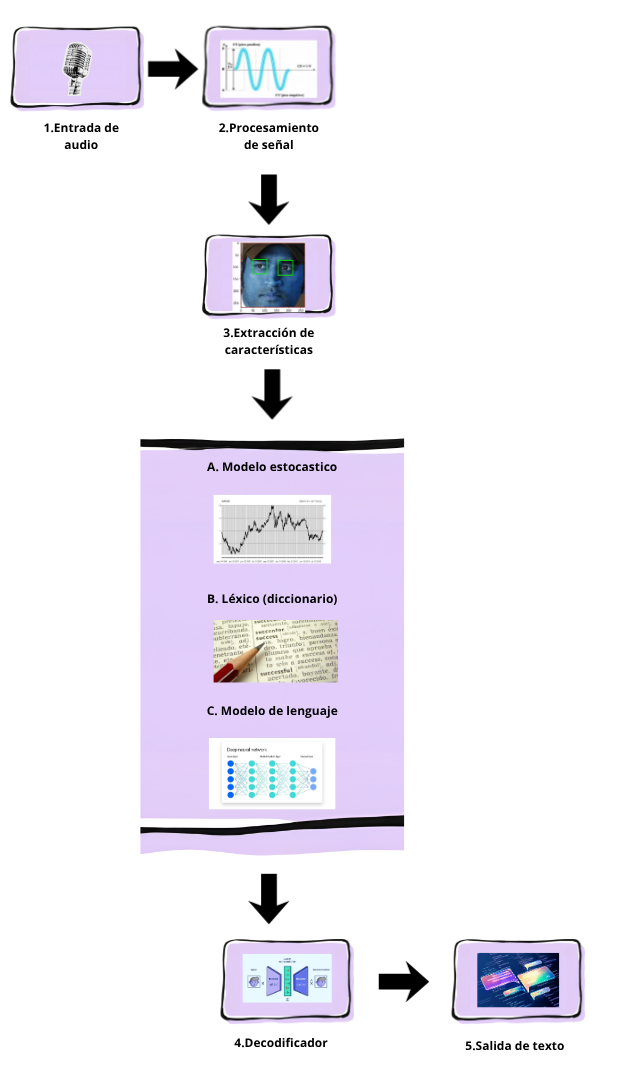
\includegraphics[width=0.7\textwidth]{img1.png} 
			\caption{Esquema de los componentes de un sistema de reconocimiento de voz.}
			\label{fig:esquema_1}
		\end{figure}	 
		
		\item{Explica, paso a paso, el flujo de cálculo de los coeficientes MFCC (pre-énfasis, ventaneo, DFT, filtros Mel,log, DCT).}
		
		
		\begin{itemize}
			\item {Pre-énfasis}  \\ 
			Se aplica un filtro de paso alto a la señal de audio original para equilibrar el espectro, ya que los sonidos humanos concentran la mayor parte de su energía natural en las bajas frecuencias. Esto se logra amplificando las altas frecuencias mediante la ecuación diferencial $y[t] = x[t] - \alpha x[t-1]$, donde el coeficiente $\alpha$ suele configurarse entre $0.95$ y $0.97$.
			
			\item {Enmarcado y ventaneo} 	\\
			El audio es dinámico, pero sus frecuencias son estadísticamente estables en fragmentos muy cortos (típicamente de 20 a 40 milisegundos). La señal continua se divide en estos marcos superpuestos. A cada uno se le aplica una función (como la ventana de Hamming o Hann) que atenúa los extremos del marco hacia cero. Esto evita cortes abruptos en los bordes que generarían ruido de alta frecuencia inexistente al transformarlo.
			
			\item {Transformada discreta de Fourier (DTF)} 	\\
			Se calcula la DFT (generalmente optimizada mediante el algoritmo FFT) sobre cada marco ventaneado para convertir la señal del dominio del tiempo al dominio de la frecuencia. El resultado es el espectro de magnitud, el cual revela exactamente cuánta energía existe en cada frecuencia durante ese breve lapso.
			
			\item {Banco de filtros Mel}	\\
			El oído humano discrimina con precisión los cambios tonales en las frecuencias bajas, pero agrupa las frecuencias altas. Para modelar esta biología, se aplica un banco de filtros triangulares sobre el espectro de magnitud. Estos filtros se distribuyen linealmente por debajo de los 1000 Hz y logarítmicamente en frecuencias superiores, mapeando la frecuencia real a la escala perceptual Mel mediante la relación $m = 2595 \log_{10}(1 + \frac{f}{700})$.		
			
			
			\item {Logaritmo}	\\	
			
			Se obtiene el logaritmo natural o en base 10 de las energías resultantes en cada filtro Mel. Esto emula la respuesta acústica del oído a los cambios de volumen (que también es logarítmica) y convierte el producto matemático de la señal original (la vibración de las cuerdas vocales) y su modulación (la forma del tracto vocal) en una simple suma lineal, facilitando su separación.
			
			
			\item {Transformada de Coseno Discreta (DCT) } \\
			
			Dado que los filtros Mel se solapan, sus bandas de energía adyacentes quedan altamente correlacionadas. La DCT se aplica sobre el logaritmo de las energías para descorrelacionar las características y concentrar la información estructural más importante en los primeros coeficientes. Se descartan las fluctuaciones rápidas (coeficientes superiores) y se conservan únicamente los primeros 12 a 13 valores que constituyen el vector MFCC final por marco.
			
			
		\end{itemize}	
		
		
		\begin{enumerate}
			\item \textbf{Investiga y compara dos algoritmos de búsqueda usados en decodificación: Viterbi y Beam Search.}
			
			Ambos algoritmos resuelven el problema de encontrar la secuencia de estados ocultos más probable $Q = \{q_1, q_2, \dots, q_T\}$ dada una secuencia de observaciones $O = \{o_1, o_2, \dots, o_T\}$, pero difieren drásticamente en su enfoque de optimización.
			
			\begin{itemize}
				\item \textbf{Viterbi:} \\
				Es un algoritmo exacto basado en programación dinámica que garantiza encontrar el óptimo global (la secuencia absoluta más probable). Calcula iterativamente la probabilidad máxima de llegar al estado $j$ en el instante de tiempo $t$:
				\begin{equation}
					\delta_t(j) = \max_{1 \le i \le N} [\delta_{t-1}(i) a_{ij}] b_j(o_t)
				\end{equation}
				donde $a_{ij}$ es la probabilidad de transición del estado $i$ al $j$, y $b_j(o_t)$ es la probabilidad de emisión. Almacena el argumento máximo de cada paso en una matriz y, al finalizar la secuencia temporal, realiza \textit{backtracking} para recuperar el camino óptimo. Su complejidad espacial y temporal es alta: $\mathcal{O}(N^2 \cdot T)$.
				
				\item \textbf{Beam Search:} \\
				Es un algoritmo heurístico (codicioso adaptativo) de búsqueda por haces. En lugar de evaluar todos los $N$ estados posibles en cada instante $t$, solo conserva las $k$ rutas (hipótesis) más probables, donde $k$ es el \textit{beam width} (ancho del haz). 
				\begin{equation}
					\text{Hipótesis conservadas en } t = top\text{-}k \left( P(q_t | q_{t-1}, O) \right)
				\end{equation}
				Descarta el resto de los caminos (poda). Esto reduce la complejidad a $\mathcal{O}(k \cdot T)$, ahorrando gran cantidad de memoria y cómputo computacional. La desventaja es que pierde la garantía matemática de encontrar el óptimo global absoluto.
			\end{itemize}
			
			\vspace{0.5cm}
			\item \textbf{Propón un experimento donde se prueben distintas técnicas de extracción de características (MFCC vs LPC vs Wavelets).}
			
			\textbf{Experimento: Sistema de Reconocimiento de Dígitos Aislados} \\
			El objetivo es evaluar el impacto de los descriptores acústicos sobre un clasificador unificado utilizando el \textit{Free Spoken Digit Dataset} (FSDD).
			
			\begin{itemize}
				\item \textbf{Preprocesamiento:} Aplicar \textit{Voice Activity Detection} (VAD) para recortar silencios y normalizar la amplitud $x[n]$ al rango $[-1, 1]$.
				\item \textbf{Extracción de Características (Variables Independientes):} Se crearán tres conjuntos de datos, procesando la señal con ventanas solapadas:
				\begin{itemize}
					\item \textit{MFCC:} Extraen la envolvente espectral modelando la percepción humana. Transformación a la escala Mel:
					\begin{equation}
						m = 2595 \log_{10}\left(1 + \frac{f}{700}\right)
					\end{equation}
					\item \textit{LPC (Codificación Predictiva Lineal):} Modelan la física del tracto vocal y sus resonancias, asumiendo que la muestra actual es una suma ponderada de $p$ muestras anteriores:
					\begin{equation}
						\hat{x}[n] = \sum_{k=1}^{p} \alpha_k x[n-k]
					\end{equation}
					\item \textit{Wavelets (DWT):} Se aplica la Transformada Discreta Wavelet mediante filtros conjugados en cuadratura (pasa-bajas $h$ y pasa-altas $g$). Proporciona un análisis multiresolución.
				\end{itemize}
				\item \textbf{Evaluación:} Entrenar el mismo modelo estadístico (ej. \textit{Support Vector Machine}) con los tres conjuntos. Se contrastarán las métricas de \textit{Accuracy} global, Precisión por clase, y los tiempos de procesamiento (\textit{Inference time}).
			\end{itemize}
			
			\vspace{0.5cm}
			\item \textbf{Describe con un ejemplo cómo se utilizarían los HMM para modelar fonemas en una palabra.}
			
			Supongamos el modelado del reconocimiento de la palabra ``UNO''. Fonéticamente, esta se compone de la secuencia de fonemas: /u/, /n/, y /o/.
			
			\begin{itemize}
				\item \textbf{Topología por Fonema:} Cada fonema se modela mediante un HMM \textit{Left-to-Right} (de izquierda a derecha), generalmente con 3 estados ocultos ($S_1, S_2, S_3$) que representan el inicio, el centro estacionario y el fin del sonido. La matriz de transición $A = [a_{ij}]$ impide el salto hacia atrás en el tiempo:
				\begin{equation}
					a_{ij} = P(q_{t+1}=S_j | q_t=S_i) = 0 \quad \forall \ j < i
				\end{equation}
				
				\item \textbf{Modelo Concatenado (La Palabra):} El HMM léxico para ``UNO'' se forma enlazando el estado de salida de un fonema con el estado de entrada del fonema subsecuente:
				\begin{equation}
					\lambda_{UNO} = HMM_{/u/} \rightarrow HMM_{/n/} \rightarrow HMM_{/o/}
				\end{equation}
				
				\item \textbf{Dinámica de Emisión y Transición:} Mientras el locutor emite el fonema /u/, el sistema genera secuencias de observaciones acústicas $O_t$ asociadas al estado central $S_2$ con una probabilidad $b_2(O_t)$. Dado que las vocales duran varios milisegundos, el modelo utilizará la auto-transición $a_{22}$ para permanecer en $S_2$. 
				
				Al cambiar biológicamente al sonido /n/, el espectro acústico cambia drásticamente. El modelo reflejará esto con un salto $a_{23}$ y posteriormente la transición de $HMM_{/u/}$ hacia $HMM_{/n/}$. Durante la decodificación de un audio real $O$, el sistema utilizará Viterbi para calcular $P(O | \lambda_{UNO})$ y determinar si esta palabra es la que mejor explica el audio capturado.
			\end{itemize}
			
		\end{enumerate}
		
		
		
		
	\end{itemize}
	
	
	
	
	\newpage
	\section{Conclusiones}
	Esta actividad permitió consolidar los fundamentos teóricos y arquitectónicos que componen un sistema de reconocimiento automático de voz (ASR). A lo largo de la investigación, quedó en evidencia que transformar una señal acústica continua en una cadena de texto discreta no es una simple traducción directa, sino un complejo problema de optimización estadística. Gracias al desglose del \textit{Front-End}, se comprendió el papel crucial de la extracción de características, como los coeficientes MFCC, los cuales modelan la audición humana y descartan información irrelevante de la señal original. Asimismo, la integración del Teorema de Bayes ilustró cómo un decodificador balancea la probabilidad acústica proveniente de un Modelo Oculto de Markov (HMM) con el contexto probabilístico de un modelo de lenguaje. En resumen, analizar algoritmos desde Viterbi hasta la estimación de Parzen demuestra el fuerte puente que existe entre el procesamiento digital de señales y el aprendizaje probabilístico moderno.
	
	\newpage
	\section{Referencias}
	\begin{itemize}
		\item Jurafsky, D., \& Martin, J. H. (2024). \textit{Speech and Language Processing} (3rd ed. draft). Stanford University.
		\item Rabiner, L. R., \& Juang, B. H. (1993). \textit{Fundamentals of Speech Recognition}. Prentice-Hall, Inc.
		\item Huang, X., Acero, A., \& Hon, H. W. (2001). \textit{Spoken Language Processing: A Guide to Theory, Algorithm, and System Development}. Prentice Hall PTR.
		\item O'Shaughnessy, D. (2000). \textit{Speech Communications: Human and Machine} (2nd ed.). IEEE Press.
	\end{itemize}
\end{document}